\section*{Math 202A - Final Exam - Dan Davison - \texttt{ddavison@berkeley.edu}}

\begin{mdframed}
  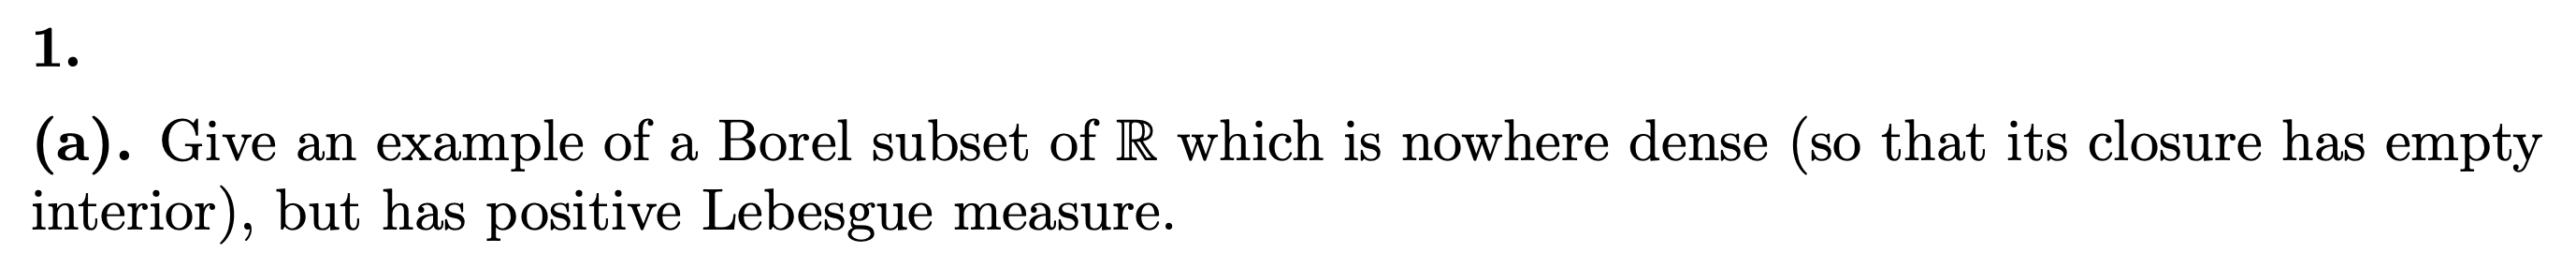
\includegraphics[width=400pt]{img/analysis--berkeley-202a-final-c9d2.png}
\end{mdframed}
\green{COMPLETE}

\begin{proof}
  The ``fat Cantor set​'' is an example of such a set. The fat Cantor set of measure $a \in (0, 1)$ is formed as
  follows:

  Note that $\sum_{n=1}^\infty \frac{1 - a}{2^n} = 1 - a$. So we will design an algorithm that
  removes $\frac{1-a}{2^n}$ at each iteration, for $n=1, 2, \ldots$. Note that at the start of iteration $n$
  there are $2^{n-1}$ intervals. So we remove
  \begin{align*}
    \frac{1-a}{2^{n}}\cdot\frac{1}{2^{n-1}} = \frac{1 - a}{2^{2n - 1}}
  \end{align*}
  from each interval.

  For example, to create a set with measure $a = \frac{1}{2}$,
  remove $\frac{1}{4} + 2(\frac{1}{16}) + 4(\frac{1}{64}) + \cdots = \frac{1}{2}$.
\end{proof}

\begin{mdframed}
  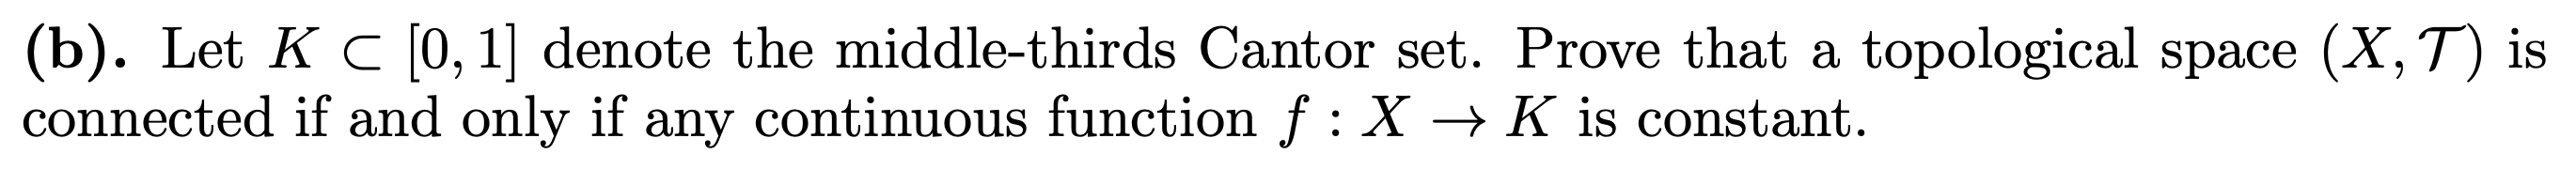
\includegraphics[width=400pt]{img/analysis--berkeley-202a-final-4333.png}
\end{mdframed}
\green{COMPLETE}

\begin{lemma}\label{cantor-set-totally-disconnected}
  Let $k_1, k_2 \in K \subset \R$ with $k_1 \neq k_2$. Then $\{k_1\}$ and $\{k_2\}$ are connected subsets,
  and $[k_1, k_2]$ is disconnected.
\end{lemma}

\begin{proof}
  Let $k_1, k_2 \in K \subset \R$ with $k_1 \neq k_2$. Without loss of generality suppose that $k_1 < k_2$.
  Then there exists $x \in K^c$ such that $k_1 < x < k_2$ (\red{TODO} I hope we proved this in class?).
  Then $[k_1, x) \isect K$ and $(x, k_2] \isect K$ are non-empty open subsets of $K$ whose union
  equals $[k_1, k_2]$, therefore $[k_1, k_2]$ is disconnected.
\end{proof}

\begin{proof}
  We view the middle-thirds Cantor set $K$ as a topological space with the topology induced by the standard
  metric on $\R$.

  $\implies$\\
  For the forwards implication, let $(X, \mc T)$ be a connected topological space and suppose for a
  contradiction that $f: X \to K$ is continuous but not constant.

  Then there exist $k_1, k_2 \in f(X)$ with $k_1 \neq k_2$. But from lemma
  \ref{cantor-set-totally-disconnected} we have that $[k_1, k_2]$ is disconnected. Therefore $f(X)$ is
  disconnected. But by Bass theorem 20.48 the image of a connected topological space under a continuous map
  between topological spaces is connected, and so this is a contradiction. Therefore if $f$ is continuous it
  must be constant.

  $\impliedby$\\
  For the reverse implication, let every continuous function $f: X \to K$ be constant and suppose for a
  contradiction that $(X, \mc T)$ is not connected.

  Let $G_1, G_2 \subset X$ be non-empty disjoint open subsets of $X$ such that $G_1 \union G_2 = X$.
  Let $H_1, H_2 \subset K$ be disjoint open subsets of $K$, and let $k_1 \in H_1$ and $k_2 \in H_2$. (\red{TODO}:
  prove that there are two disjoint open subsets of the Cantor set.)

  Define $f: X \to K$ by
  \begin{align*}
    f(x) =
    \begin{cases}
      k_1, & x \in G_1 \\
      k_2, & x \in G_2.
    \end{cases}
  \end{align*}
  Then $f$ is not constant. Furthermore, the preimage of every open subset of $K$ is open,
  since $f^{-1}(H_1) = G_1$ and $f^{-1}(H_2) = G_2$ and $f^{-1}(H) = \emptyset$ for every open subset $H$
  of $K$ such that $H \neq H_1$ and $H \neq H_2$. Therefore $f$ is continuous. This contradicts our premise and
  thus proves that $(X, \mc T)$ is connected.
\end{proof}

\newpage
\begin{mdframed}
  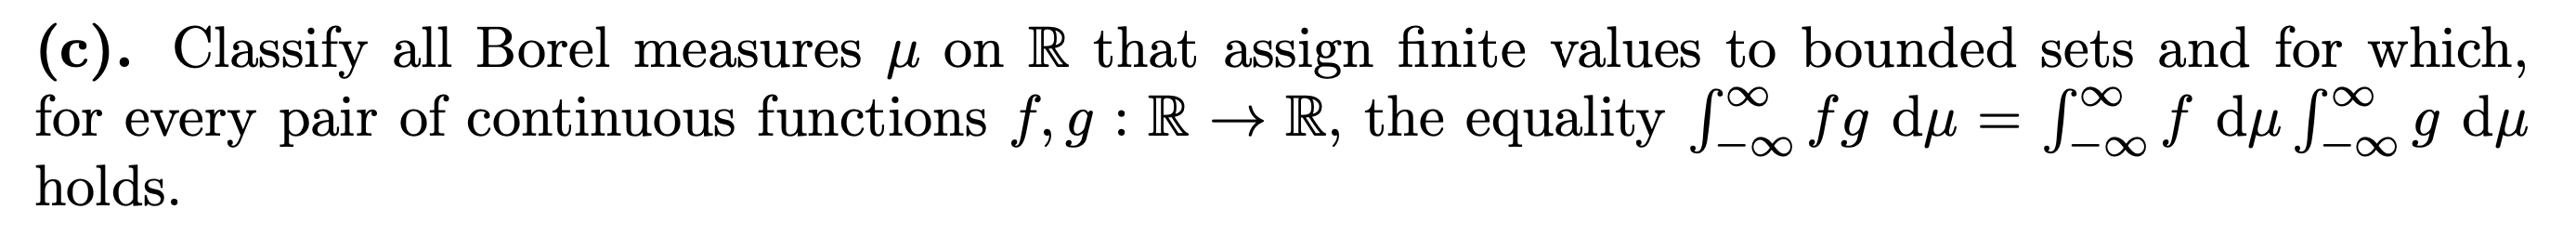
\includegraphics[width=400pt]{img/analysis--berkeley-202a-final-0bf8.png}
\end{mdframed}

% https://math.stackexchange.com/questions/2250993/when-the-integral-of-products-is-the-product-of-integrals

\begin{proof}
  Let $\mc M$ be the collection of all Borel measures $\mu$ on $\R$ that satisfy both the following conditions:
  \begin{enumerate}
  \item $\mu(A) < \infty$ for every bounded set $A \subset \R$
  \item $\int_{-\infty}^\infty fg \dmu = \(\int_{-\infty}^\infty f \dmu\) \(\int_{-\infty}^\infty g \dmu\)$ for every pair $f, g: \R \to \R$ of continuous functions.
  \end{enumerate}

  We are asked to ``classify​'' this collection.

  I think this might mean to specify an equivalence relation on $\mc M$ and perhaps also, if the
  number of equivalence classes is finite and small, give an example member of each.

  The second condition (that integration commutes with pointwise multiplication of continuous
  functions) is interesting. It reminds me of an orthogonality or independence condition, i.e. it
  seems that in some sense the measure is such that for every pair $f, g$ of continuous
  functions $f$ and $g$ don't ``interact​''.

  For example, if $\mu$ is a probability measure on $\R$ (for example, the Gaussian probability
  measure) and if $f$ and $g$ are independent random variables then (Bass theorem 21.10)
  \begin{align*}
    \mathbb{E}(XY)
    &= \int_0^\infty fg \dmu \\
    &= \(\int_0^\infty f \dmu\) \(\int_0^\infty g \dmu\) \\
    &= \mathbb{E}(X)\mathbb{E}(Y).
  \end{align*}
  However, in order for this line of thinking to be relevant, we would need to explain the
  connection between continuity of $f$ and $g$ and their independence as random variables. But of
  course we could have $f = g$ and then they wouldn't be independent. It's like we're looking for
  probability measures under which every random variable is independent.

  So an example of a measure that does satisfy these conditions is the Dirac measure: for
  given $x \in \R$ the measure is defined by $\delta_x(A) = 1$ if $x \in A$ and $0$ otherwise. It
  assigns a finite value to every set, and therefore to every bounded set, and we have
  \begin{align*}
    \int_{-\infty}^\infty fg \d\delta_x = f(x)g(x) = \(\int_{-\infty}^\infty f \d\delta_x\) \(\int_{-\infty}^\infty g \d\delta_x\).
  \end{align*}
  Are there any other measures that satisfy the conditions?

  Suppose $\mu$ is such a measure. Then
  \begin{align*}
    \int_{-\infty}^\infty fg \dmu = \(\int_{-\infty}^\infty f \dmu\) \(\int_{-\infty}^\infty g \dmu\)
  \end{align*}
  for every pair $f, g: \R \to \R$ of continuous functions. But I'm not sure where to go from here.

  I'm going to conjecture without proof that there is an equivalence relation on the collection of
  measures specified in the question and that every equivalence class has a canonical
  representative which is a probability measure with the property that every pair of random
  variables is independent (even two copies of the same random variable), and that in fact the
  Dirac measure is the only such probability measure.
\end{proof}

\newpage
\begin{mdframed}
  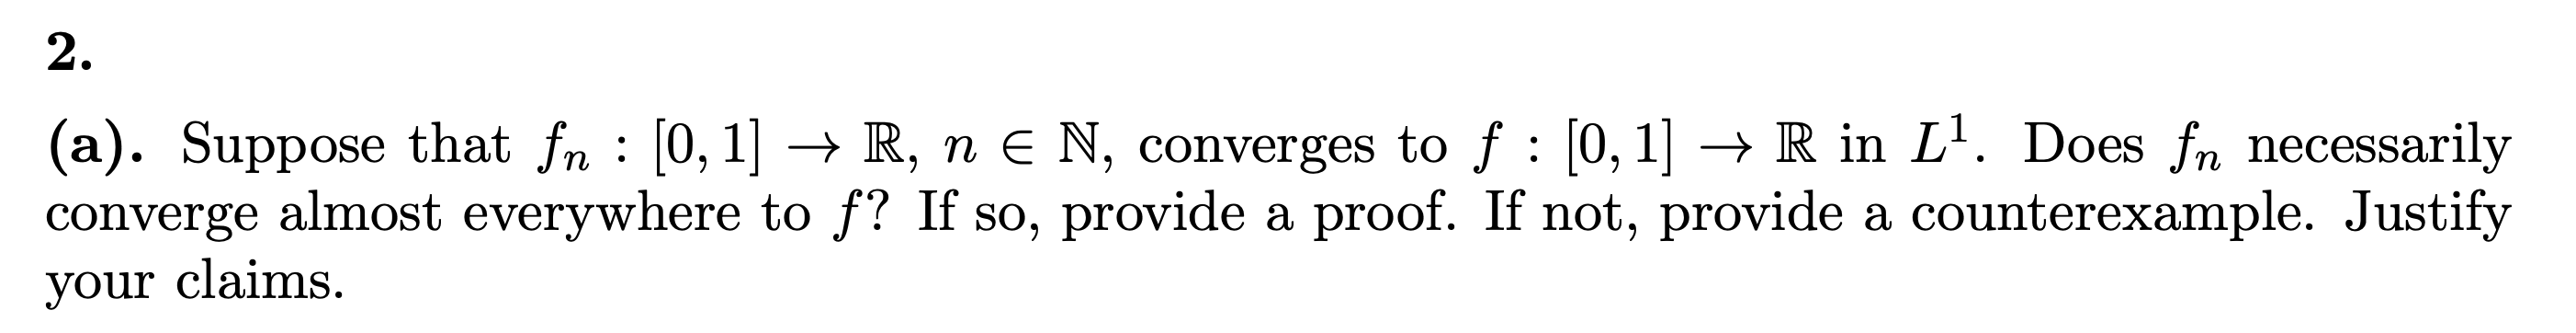
\includegraphics[width=400pt]{img/analysis--berkeley-202a-final-04b9.png}
\end{mdframed}
\green{COMPLETE}

\begin{proof}
  $f_n$ does not necessarily converge almost everywhere to $f$. Bass Example 10.7 is a counter example. I'm
  just going to copy it here rather than type it out myself, but I did do some thinking about this before
  consulting external sources (below).
  \begin{mdframed}
    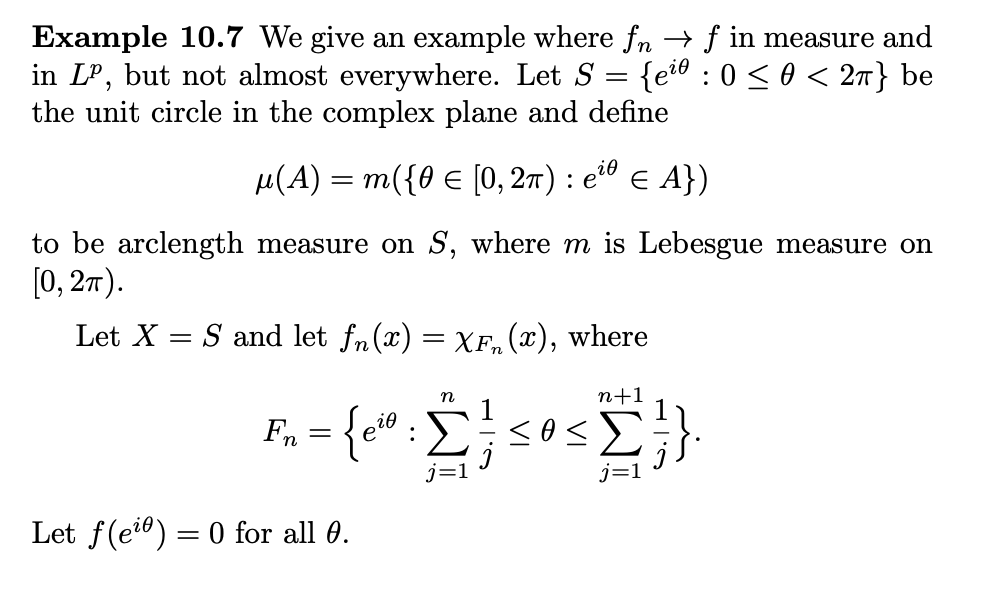
\includegraphics[width=200pt]{img/analysis--berkeley-202a-final-35f7.png}\\
    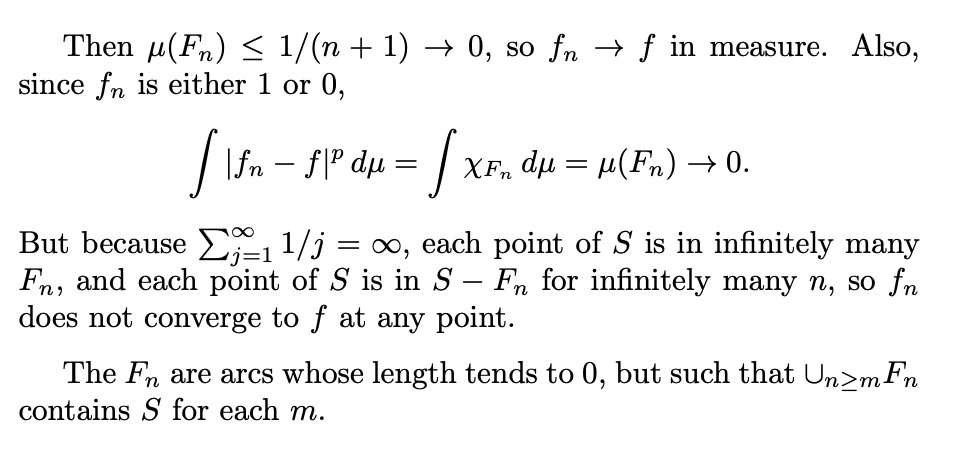
\includegraphics[width=200pt]{img/analysis--berkeley-202a-final-07d9.png}
  \end{mdframed}
\end{proof}

\red{The above counterexample from Bass is the correct answer. However here is some thinking I
  did about this independently prior to consulting Bass.}

Let $f_n: [0, 1] \to \R$ be a sequence of functions converging to $f: [0, 1] \to \R$ in $L^1$.

Let $E \subseteq [0, 1]$ be the set of points at which $f_n$ does not converge to $f$. Suppose for a
contradiction that $\mu(E) > 0$.

Since $f_n \to f$ in $L^1$ we have $\limninf \int |f_n - f| = 0$. Therefore $\limninf \int_E |f_n - f| = 0$.

I think that's not possible and therefore a contradiction proving that $f_n \to f$ almost everywhere.

(No, this is wrong -- see above)

One might think that the sequences $f_n(x)$ for $x \in E$ could contrive to, at every
generation $n$, almost all be exactly equal to $f(x)$, except for a negligible ``error set​'', with
membership of this error set changing over time such that every $x \in E$ will at some point in the
future be a member of the error set again, in which case there would be convergence nowhere while
retaining $\limninf \int_E |f_n - f| = 0$. However, if only a negligible set is allowed to
participate in the error set at every generation $n$, then it is impossible for all the elements of
a positive measure set to participate in the error set over the course of countably many
generations.

So it seems that this might be a contradiction, but we need to prove it.

Set $d_n = |f_n - f|$ and let $\eps > 0$. Since $\int_E d_n \to 0$ there exists $N$ such
that $\int_E d_n < \eps$ for all $n \geq N$. Let $n \geq N$. \red{(incomplete, and doomed; see above.)}

% \begin{theorem}[Bass proposition 8.1]\label{bass-8.1}
%   If $f$ is real-valued, non-negative, and measurable, and $\int f = 0$, then $f = 0$ a.e.
% \end{theorem}

% \begin{proof}
%   \red{TODO}
%   Let $f_n: [0, 1] \to \R$, $n \in \N$, converge to $f: [0, 1] \to \R$ in $L^1$. Thus, by definition,
%   \begin{align*}
      %       \limninf \int |f_n - f| = 0.
      %     \end{align*}
      %       We want to prove or disprove the statement
      %       \begin{align*}
      %       \limn f_n = f \ae
      %     \end{align*}
      %       Suppose we could bring the limit inside. Then
      %       \begin{align*}
      %       \int \limninf |f_n - f| = 0,
      %     \end{align*}
      %       therefore by Bass proposition 8.1 $\limninf |f_n - f| = 0$ a.e. and thus $f_n$ converges almost everywhere to $f$.

      %       But bringing the limit inside is justified by neither MCT nor DCT. So let's look for a counter-example based
      %       on not satisfying DCT conditions.
      %       \end{proof}

\newpage
\begin{mdframed}
  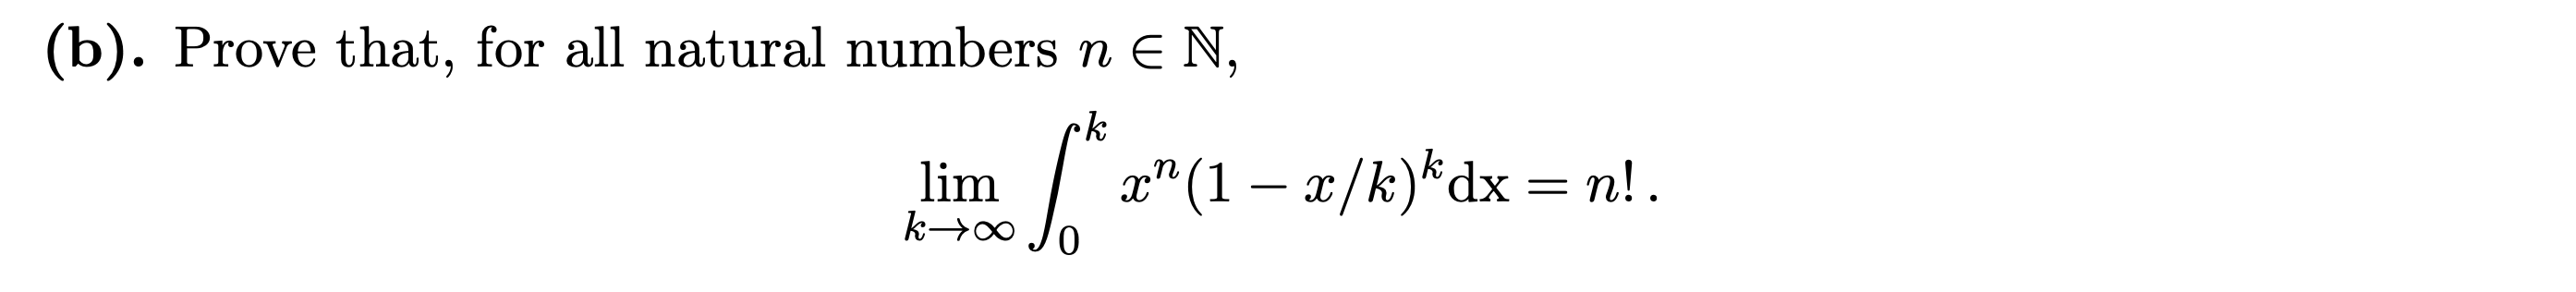
\includegraphics[width=400pt]{img/analysis--berkeley-202a-final-96cc.png}
\end{mdframed}
\green{COMPLETE}

I think my proof is put on a slightly firmer basis if I say at the outset that the syntax $e^{-x}$
is defined to mean the Maclaurin expansion: $e^{-x} := \sum_{j=0}^\infty (-1)^j ~ \frac{x^j}{j!}$.

\begin{definition*}
  Define Euler's gamma function $\Gamma: \R \to \R$
  by $\Gamma(y + 1) = \int_0^\infty x^y e^{-x} \dx$.
\end{definition*}

\begin{lemma}\label{gamma-function}
  $\Gamma(n + 1) = n!$ for $n \in \N$.
\end{lemma}

\begin{proof}
  Integration by parts (with $u = x^n$, $\dvdx = e^{-x}$) yields
  \begin{align*}
    \Gamma(y + 1)
    &= \big[-x^ye^{-x}\big]_0^\infty + y\int_0^\infty x^{y-1}e^{-x} \dx \\
    &= y\Gamma(y),
  \end{align*}
  since $x^ye^{-x} \to 0$ as $x \to \infty$.

  We have $\Gamma(1) = \int_0^\infty e^{-x} \dx = 1$, and therefore $\Gamma(n + 1) = n!$
  for $n \in \N$.

  (Since these are continuous functions, Lebesgue and Riemann integrals coincide and we freely use
  standard results for antiderivatives and derivatives from introductory calculus).
\end{proof}

\begin{lemma}\label{exponential-limit}
  $(1 - x/k)^k < e^{-x}$ for all $k \in \N$ and all $x \in \R$
  and $\lim_{k \to \infty} \(1 - \frac{x}{k}\)^k = e^{-x}$.
\end{lemma}

\begin{proof}
  Recall the Maclaurin expansion $e^{-x} = \sum_{j=0}^\infty (-1)^j ~ \frac{x^j}{j!}$ and observe that
  \begin{align*}
    \(1 - \frac{x}{k}\)^k
    &= \sum_{j=0}^k {k \choose j} \(\frac{-x}{k}\)^j \\
    &= \sum_{j=0}^k (-1)^j \frac{x^j}{j!} \(\frac{k!/(k-j)!}{k^j} \) \\
    & <\sum_{j=0}^k (-1)^j \frac{x^j}{j!}.
  \end{align*}
  Therefore $(1 - x/k)^k < e^{-x}$ for all $k \in \N$ and all $x \in \R$.

  Furthermore we have
  \begin{align*}
    \lim_{k \to \infty} \(1 - \frac{x}{k}\)^k
    &= \sum_{j=0}^\infty (-1)^j \frac{x^j}{j!} \(\lim_{k \to \infty} \frac{k!/(k-j)!}{k^j} \).
  \end{align*}
  Note that
  \begin{align*}
    \lim_{k \to \infty} \frac{k!/(k-j)!}{k^j}
    &= \lim_{k \to \infty} \frac{k   (k - 1)     (k - 2)       \cdots (k - (j - 1))}{k^j} \\
    &= \lim_{k \to \infty} \frac{k^j (1 - k^{-1}) (1 - 2k^{-1}) \cdots (1 - (j - 1)k^{-1})}{k^j} \\
    &= 1,
  \end{align*}
  therefore $\lim_{k \to \infty} \(1 - \frac{x}{k}\)^k = e^{-x}$.
\end{proof}

\begin{claim*}
  $\lim_{k \to \infty} \int_0^k x^n (1 - x/k)^k \dx= n!$ for all $n \in \N$.

\end{claim*}

\begin{proof}
  We may apply the dominated convergence theorem, since the integrand $x^n (1 - x/k)^k$ is
  non-negative and by lemma \ref{exponential-limit} is bounded above by $x^ne^{-x}$ which as shown
  in lemma \ref{gamma-function} is integrable.

  Therefore
  \begin{align*}
    \lim_{k \to \infty} \int_0^k x^n (1 - x/k)^k \dx
    &= \lim_{k \to \infty} \int_0^\infty x^n (1 - x/k)^k\ind_{[0, k]} \dx \\
    &= \int_0^\infty x^n \lim_{k \to \infty} (1 - x/k)^k\ind_{[0, k]} \dx & \text{by the dominated convergence theorem}\\
    &= \int_0^\infty x^n e^{-x} \dx & \text{by lemma \ref{exponential-limit}}\\
    &=: \Gamma(n + 1) \\
    &= n!  & \text{by lemma \ref{gamma-function}}.\\
  \end{align*}
\end{proof}

\red{TODO: What did this have to do with part (a)?}

\newpage
\begin{mdframed}
  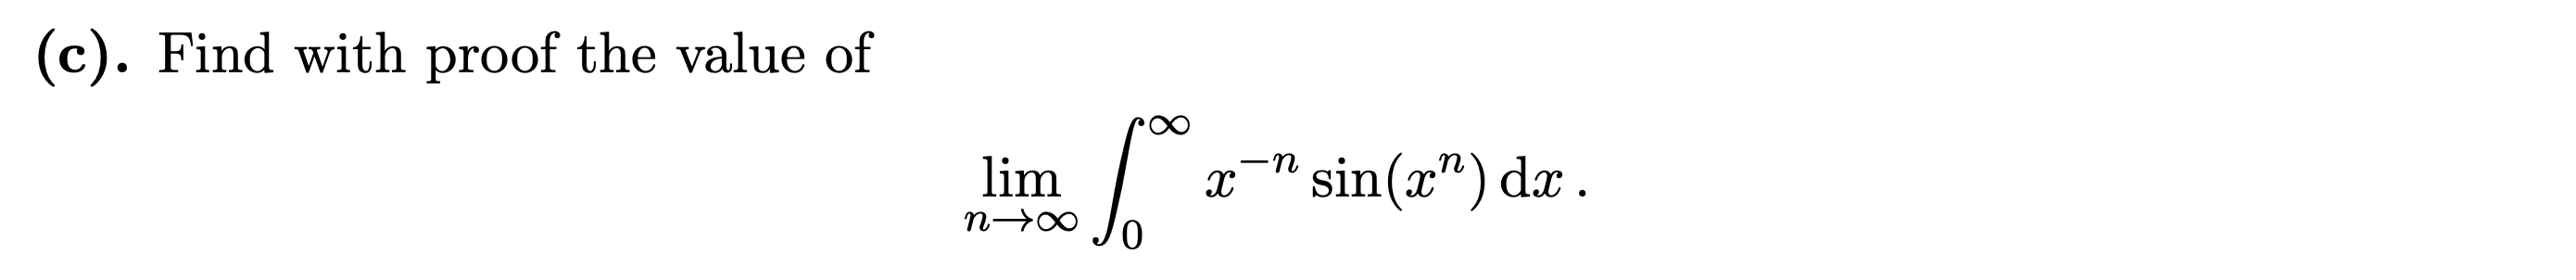
\includegraphics[width=400pt]{img/analysis--berkeley-202a-final-c137.png}
\end{mdframed}
\green{COMPLETE}

\begin{proof}
  Define $f_n = x^{-n}\sin(x^n)$ for $n \geq 2$. We have
  \begin{align*}
    \limninf \int_0^\infty f_n(x) \dx
    &= \limninf \(\int_0^1 f_n(x) \dx + \int_1^\infty f_n(x) \dx\) \\
    &= \limninf \int_0^1 f_n(x) \dx + \limninf \int_1^\infty f_n(x) \dx.
  \end{align*}
  Note that $|x^{-n}\sin(x^n)|$ on $[0, 1)$ is bounded above by $1$, which is integrable, so we can apply the dominated
  convergence theorem, yielding
  \begin{align*}
    \limninf \int_0^1 x^{-n}\sin(x^n) \dx = \int_0^1 \limninf  x^{-n}\sin(x^n) \dx.
  \end{align*}
  Since $\limninf x^{n} = \limninf \sin(x^n) = 0$ for $x \in [0, 1)$ we can apply l'Hopital's rule,
  yielding
  \begin{align*}
    \int_0^1 \limninf  x^{-n}\sin(x^n) \dx
    = \int_0^1 \limninf \frac{nx^{n-1}\cos(x^n)}{nx^{n-1}} \dx
    = 1.
  \end{align*}
  Also $\limninf \int_1^\infty x^{-n}\sin(x^n) \dx = 0$ is for $n \geq 2$ bounded above
  by $x^{-2}$, which is integrable, so we can again apply the dominated convergence theorem,
  yielding
  \begin{align*}
    \limninf \int_1^\infty x^{-n}\sin(x^n) \dx
    &= \int_1^\infty \limninf x^{-n}\sin(x^n) \dx.
  \end{align*}
  Now we
  have $\limsup_{n \to \infty} x^{-n}\sin(x^n) = \liminf_{n \to \infty} x^{-n}\sin(x^n) = 0$,
  hence $\limninf x^{-n}\sin(x^n) = 0$, hence $\int_1^\infty \limninf x^{-n}\sin(x^n) \dx = 0$.

  Therefore we have $\limninf \int_0^1 f_n(x) \dx = 1$ and $\limninf \int_1^\infty f_n(x) \dx = 0$,
  hence $\limninf \int_0^\infty f_n(x) \dx = 1$.
\end{proof}

% \begin{proof}
%   Let $u(x) = x^n$ so that $\dudx = nx^{n-1}$, hence $\dx = n^{-1}x^{1 - n} \du$ and
%   \begin{align*}
%     \int_0^\infty x^{-n}\sin(x^n) \dx
%     &=  n^{-1}\int_0^\infty u^{-1}\sin(u) x^{1-n} \du
% \end{align*}
% \end{proof}

% \begin{proof}
%   \begin{align*}
%     \int \sin(x^n) \dx
%     &= \int \sin(u(x)) \dxdu \du
%   \end{align*}

%   Integration by parts (with $u(x) = \sin(x^n)$, $\dvdx = x^{-n}$,
%   thus $\dudx = nx^{n-1}\cos(x^n)$, $v(x) = \frac{1}{1-n}x^{1-n}$) yields
%   \begin{align*}
%     \int_0^\infty x^{-n} \sin(x^n)
%     &= \Big[\frac{1}{1-n}\sin(x^n)x^{1-n}\Big]_0^\infty - \int_0^\infty \frac{1}{1-n}x^{1-n} nx^{n-1}\cos(x^n) \dx \\
%     &=  -\frac{n}{1-n}\int_0^\infty \cos(x^n) \dx \\
%     &=  -\cos(\frac{\pi}{2n})\Gamma(1 + \frac{1}{n}) \dx \\
%   \end{align*}

%   \begin{minted}{wolfram} :results latex
%     Integrate[x^{-n} * Sin[x^n], {x, 0, Infinity}]
%   \end{minted}

%   \begin{align*}
%     \left\{\text{ConditionalExpression}\left[-\frac{\cos \left(\frac{\pi }{2 n}\right) \Gamma \left(\frac{1}{n}-1\right)}{n},\frac{1}{2}<\Re(n)<1\land \Im(n)=0\right]\right\}
%   \end{align*}



%   \begin{minted}{wolfram} :results latex
%     Integrate[Cos[x^n], {x, 0, Infinity}]
%   \end{minted}

%   \begin{align*}
%     \text{ConditionalExpression}\left[\cos \left(\frac{\pi }{2 n}\right) \Gamma \left(1+\frac{1}{n}\right),\Re(n)>1\land \Im(n)=0\right]
%   \end{align*}
% \end{proof}

% Since the same waveform repeats a countable number of times (with the x-axis scaled differently
% each time), perhaps we can compute this as a sum over countably many areas-under-waveforms.


\newpage
\begin{mdframed}
  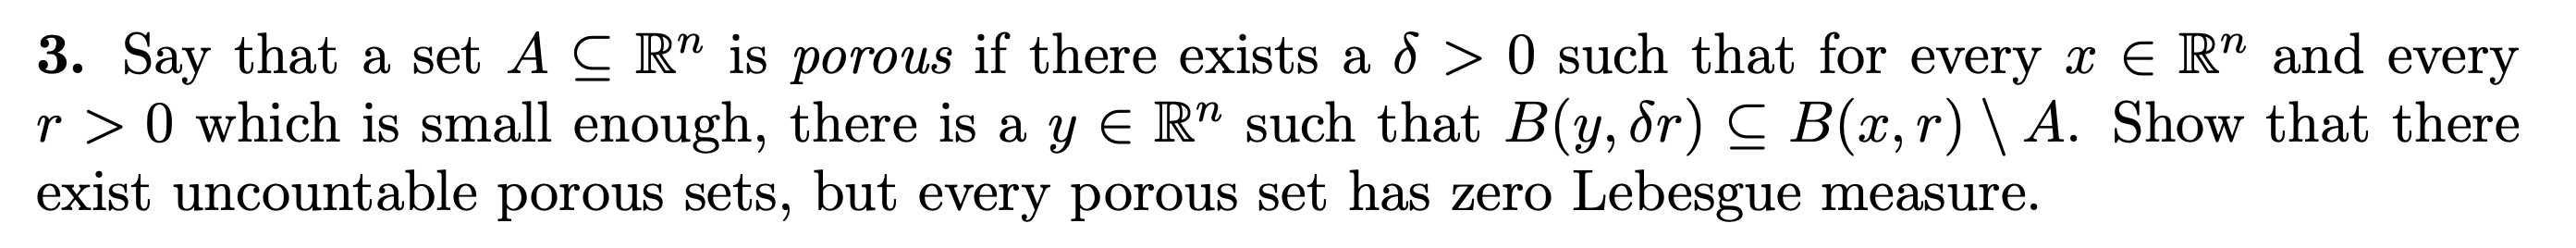
\includegraphics[width=400pt]{img/analysis--berkeley-202a-final-ef68.png}
\end{mdframed}
\green{COMPLETE}


\begin{mdframed}
  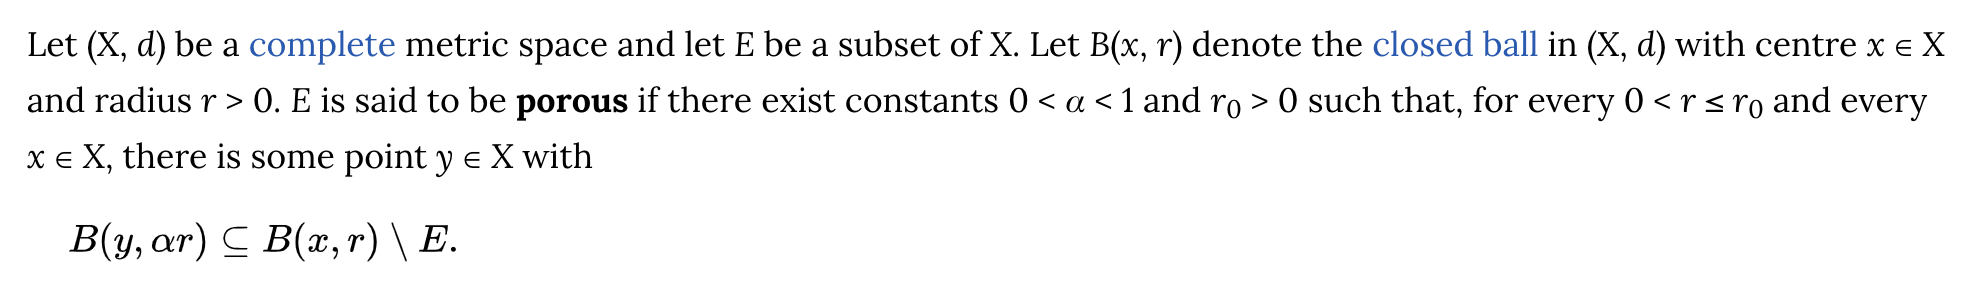
\includegraphics[width=400pt]{img/analysis--berkeley-202a-final-b463.png}
\end{mdframed}

Informally, here is what the definition says:

\begin{quote}
  For every ball (anywhere in $\R^n$) that is smaller than some fixed radius $r_0$, there exists an ``inner
  ball​'' that is smaller still by a factor of $\delta$, and which fits in the outer ball, while avoiding every
  point of $A$.
\end{quote}

Notice that in the definition, the same $\delta$ and $r_0$ work everywhere.

Consider an outer ball of size $r < r_0$. There exists an inner ball of size $\delta r$ that works. Furthermore
this inner ball works for all larger outer balls.

\begin{claim}
  There exist uncountable porous sets.
\end{claim}

\begin{proof}
  Let $A = \R \times \{0\} \subset \R^2$. Note that $A$ is uncountable, since there is an obvious bijection
  between $A$ and the uncountable set $\R$.

  Take $\delta = 1/2$ and pick any $r_0 > 0$. Let $(x, y) \in \R^2$ and let $r < r_0$.

  Suppose $y \geq 0$. Then $B\big((x, y + r/2), r/2\big) \subset B\big((x, y), r\big)$
  and $B\big((x, y + r/2), r/2\big) \isect A = \emptyset$.

  Alternatively, suppose $y < 0$. Then $B\big((x, y - r/2), r/2\big) \subset B\big((x, y), r\big)$
  and $B\big((x, y - r/2), r/2\big) \isect A = \emptyset$.

  Therefore the uncountable set $A$ is porous.
\end{proof}

\begin{claim}
  Every porous set has zero Lebesgue measure.
\end{claim}

I used the following sources in answering this question

\url{https://www.wikiwand.com/en/Porous_set}\\
\url{https://math.stackexchange.com/questions/1362464/porous-sets-why-measure-zero}\\
\url{https://www.wikiwand.com/en/Lebesgue\%27s_density_theorem}\\

\begin{proof}
  \red{TODO} (partial)

  Let $A \subseteq \R^n$ be porous, parametrized by $\delta > 0$ and $r_0 > 0$.

  Let $x \in A$ and let $y$ be such that for all $0 < r \leq r_0$ we have $B(y, \delta r) \subseteq B(x, r)$
  and $B(y, \delta r) \isect A = \emptyset$. Note that we have $m(B(y, \delta r)) < m(A^c \isect B(x, r))$.

  Now consider the ``density​'' $\frac{m(A \isect B(x, r))}{m(B(x, r))}$ of $A$ in $B(x, r)$. We have
  \begin{align*}
    \frac{m(A \isect B(x, r))}{m(B(x, r))}
    &= 1 - \frac{m(A^c \isect B(x, r))}{m(B(x, r))} \\
    &< 1 - \frac{m(B(y, \delta r))}{m(B(x, r))} \\
    &= 1 - \delta^n,
  \end{align*}
  where we have used the fact that the volume (and therefore the Lebesgue measure) of an $n$-ball of radius $r$
  is proportional to $r^n$.

  Suppose for a contradiction that $m(A) > 0$. Then by the Lebesgue density theorem we have that
  \begin{align*}
    \lim_{r \to 0} \frac{m(A \isect B(x, r))}{m(B(x, r))} = 1
  \end{align*}
  for Lebesgue-almost all points of $A$. But this is a contradiction: it implies that there exists
  a sequence $r_i \to 0$ and an $N$ such
  that $\frac{m(A \isect B(x, r))}{m(B(x, r))} > 1 - \delta^n$ for all $i > N$, whereas we showed
  above that $\frac{m(A \isect B(x, r))}{m(B(x, r))} < 1 - \delta^n$.
\end{proof}

\red{TODO: Is it correct that the Lebesgue density theorem requires the set to have positive
  measure? It seems obviously true but I couldn't see that in statements of the theorem.}


\newpage
\begin{mdframed}
  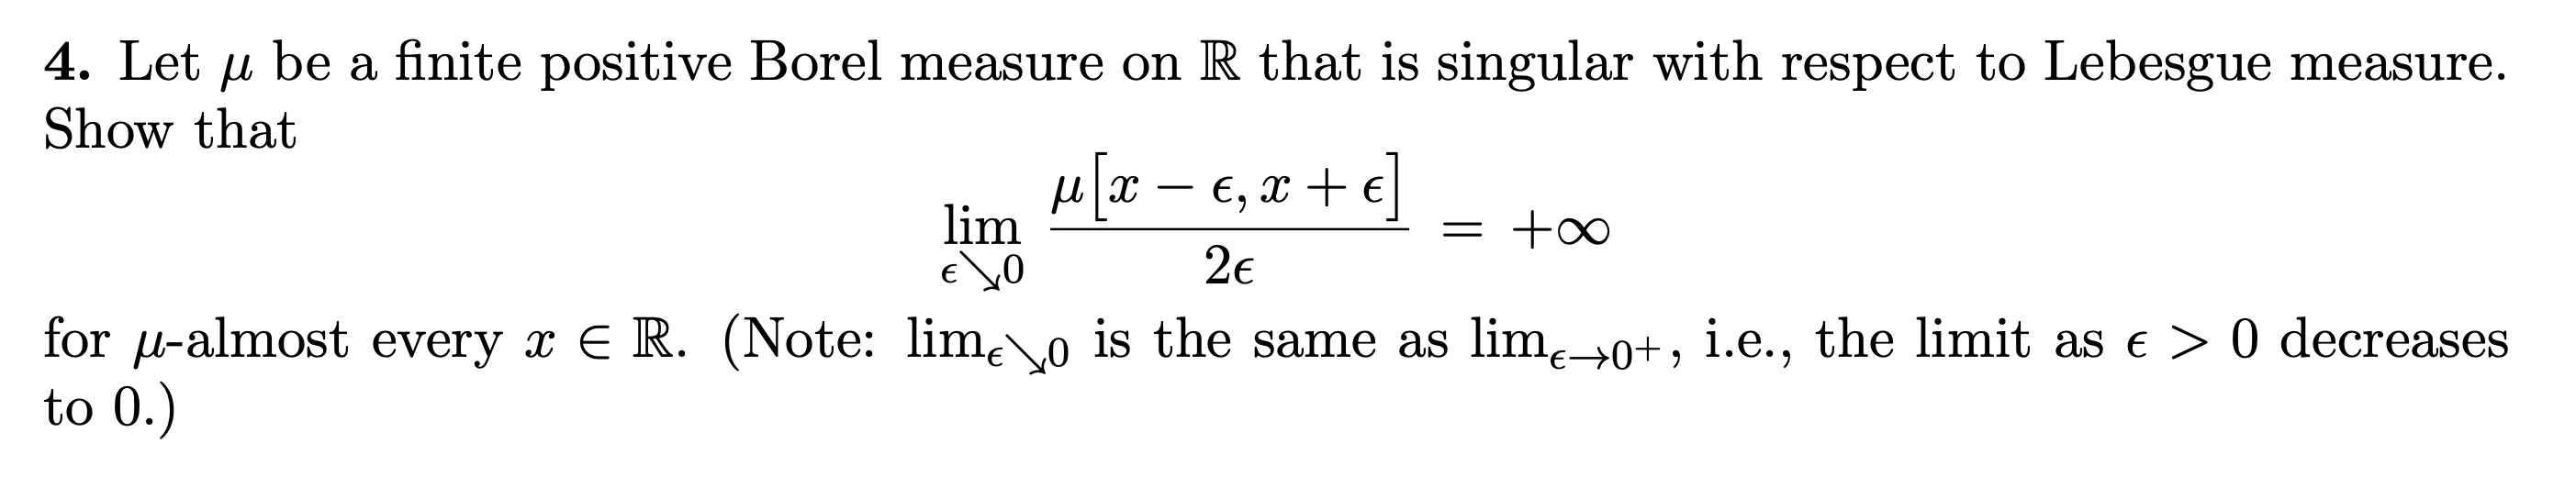
\includegraphics[width=400pt]{img/analysis--berkeley-202a-final-21a6.png}
\end{mdframed}

Let $m$ denote Lebesgue measure.

\begin{proof}
  \red{TODO} (partial)

  Since $\mu$ is singular with respect to Lebesgue measure, there exist disjoint Borel sets $U$ and $V$ such
  that $U$ is $\mu$-null and $V$ is $m$-null, and $\R = U \union V$.

  Let $0 < \mu(\R) = L < \infty$. We have
  \begin{align*}
    &\mu(U) = 0     & \mu(V) = L \\
    &m(U) = \infty & m(V) = 0,
  \end{align*}
  since by countable additivity $\infty = m(\R) = m(U) + m(V) = m(U)$,
  and $L = \mu(\R) = \mu(U) + \mu(V) = \mu(V)$.

  Note that any property that holds for all $x \in V$ holds $\mu$-almost everywhere. So let $x \in V$. We would
  like to show that
  \begin{align*}
    \lim_{\eps \searrow 0} \frac{\mu([x - \eps, x + \eps])}{2\eps} = +\infty.
  \end{align*}
  Let $\eps_n$ be a sequence converging to zero from above, let $I_n = [x - \eps_n, x + \eps_n]$, and
  let $B > 0$. We would like to show that there exists $N$ such that $\frac{\mu(I_n)}{2\eps_n} > B$ for
  all $n \geq N$.

  We have $\mu(I_n) = \mu(I_n \isect V) + \mu(I_n \isect U) = \mu(I_n \isect V)$, since $U$ is a null set
  under $\mu$. And since $x \in V$ we have $I_n \isect V \neq \emptyset$.

  If we could show that $\mu$-almost every singleton set included in $V$ has positive measure under $\mu$ then
  we would be done, since the property would hold at all of them. I think if we could show $V$ were countable
  then we'd be done for this same reason. But we can't -- e.g. the Cantor set has zero Lebesgue measure and yet
  is uncountable.

  Similarly, if we could show that there exists $N$ and $l > 0$ such that $\mu(I_n) > l$ for all $n > N$ then
  we would be done.

  Note that every interval around $x$ is not in $V$, because it has positive Lebesgue measure. In other
  words, $V$ includes no intervals. But this is true of the Cantor set also.

  \red{TODO} I don't know how to finish this.
\end{proof}

% I am assuming that the question is saying that $\mu$ and $m$ are mutually singular with respect to the
% Borel $\sigma$-algebra.

% Intuition: in some sense this question is asking us to show that the Radon-Nikodym derivative does not exist,
% because they are singular, which is sort of the opposite of absolutely continuous.

% Intuition: $\mu$ assigns positive measure to a $m$-null set. Clearly we need to show that $\mu$ assigns greater
% measure to certain intervals than $m$ does. Why is that true? Perhaps because the interval contains parts of
% an $m$-null set.

% In fact, $\mu$ only has positive measure on Lebesgue null sets. But $\mu$ does not assign positive measure to
% every singleton, since $\mu$ is finite. If we could show that $\mu$-almost every $x$ is ``surrounded by an
% arbitrarily small Lebesgue null set​'' that would do it. Perhaps the only way that makes sense is if
% $\mu$-almost every $x$ is a singleton with positive measure under $\mu$. Can we show that?

% $V$ contains no intervals, since it is Lebesgue-null. And $\mu(V) = L > 0$. This total measure $L$ is assigned
% to Lebesgue-null sets in a countably additive manner.

% \begin{mdframed}
%   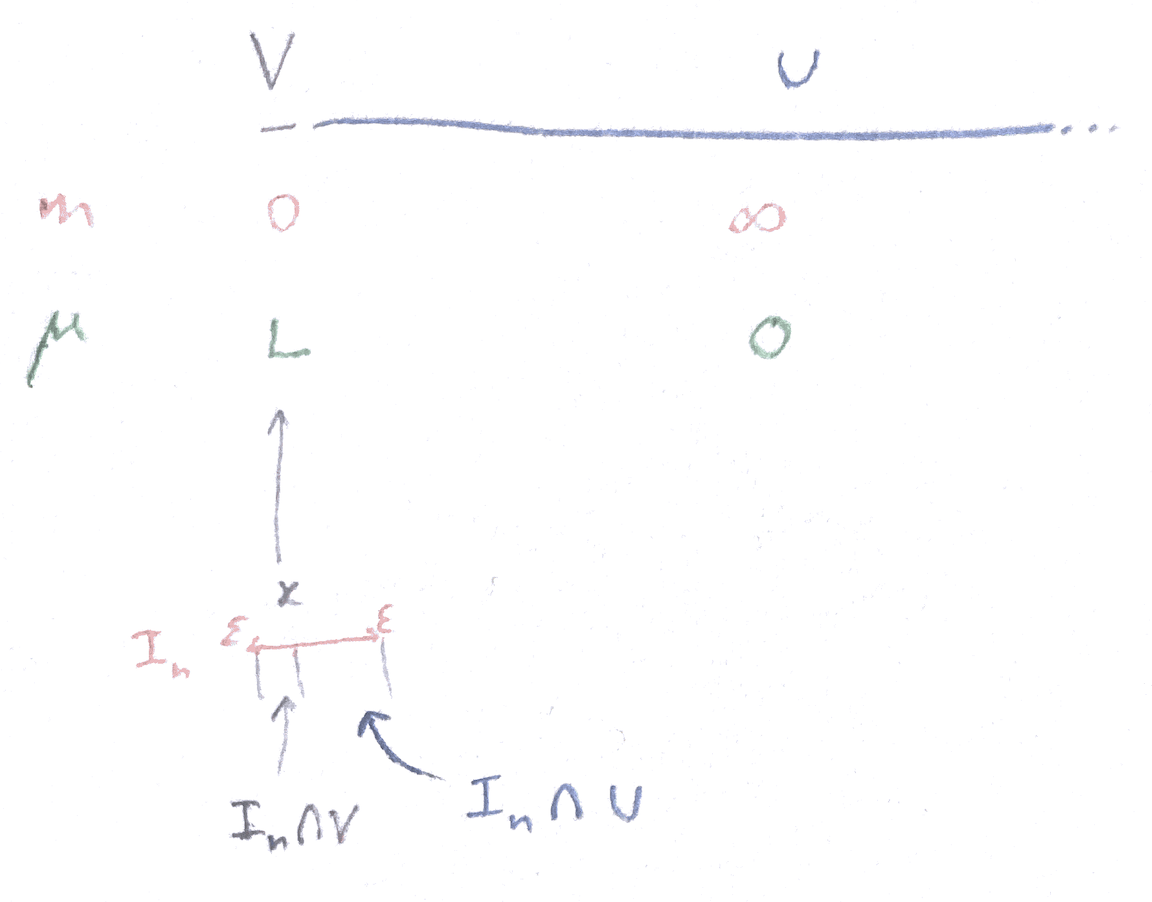
\includegraphics[width=200pt]{img/analysis--berkeley-202a-final-fe0f.png}
% \end{mdframed}



\newpage
\begin{mdframed}
  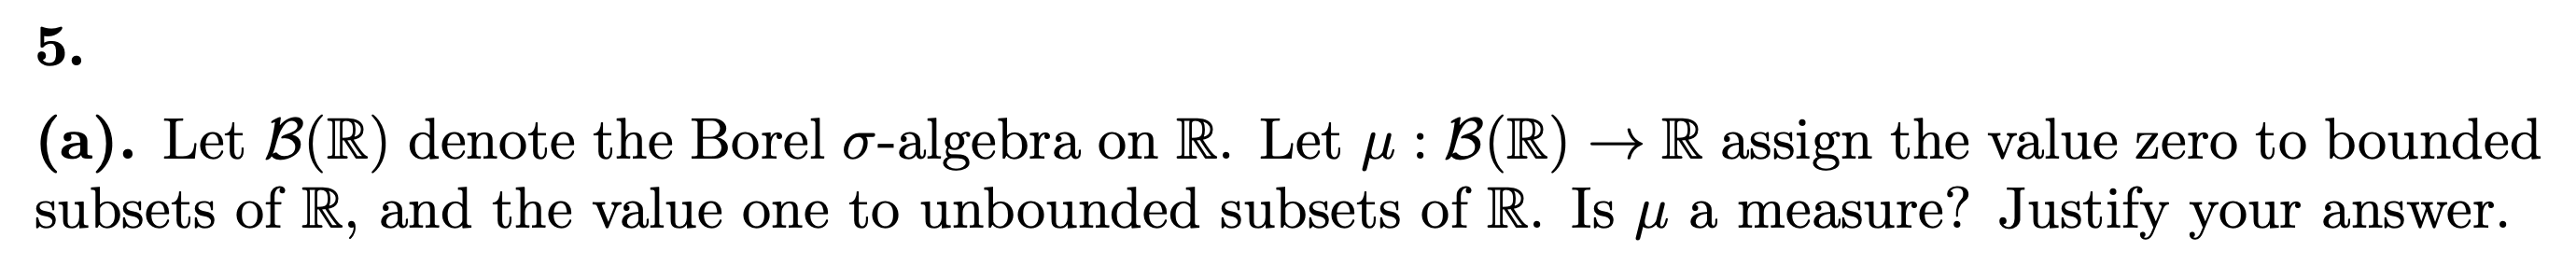
\includegraphics[width=400pt]{img/analysis--berkeley-202a-final-246a.png}
\end{mdframed}
\green{COMPLETE}

\begin{proof}

  $\mu$ is not a measure because it is not countably additive.

  To see this, let $I_n = (-n, -(n - 1)] \union [n-1, n)$, and let $\mc I = \{I_n ~:~ n \in \N\}$. Then $\mc I$
  is a pairwise disjoint, countable collection of sets and $\bigcup_{n=1}^\infty \mc I = \R$,
  therefore $\mu\(\bigcup_{n=1}^\infty \mc I\) = 1$ since $\R$ is unbounded.

  However $I_n$ is bounded for all $n$ and
  so $\sum_{n=1}^\infty \mu(I_n) = \sum_{n=1}^\infty 0 = 0 \neq \mu\(\bigcup_{n=1}^\infty \mc I\)$.
\end{proof}


\begin{mdframed}
  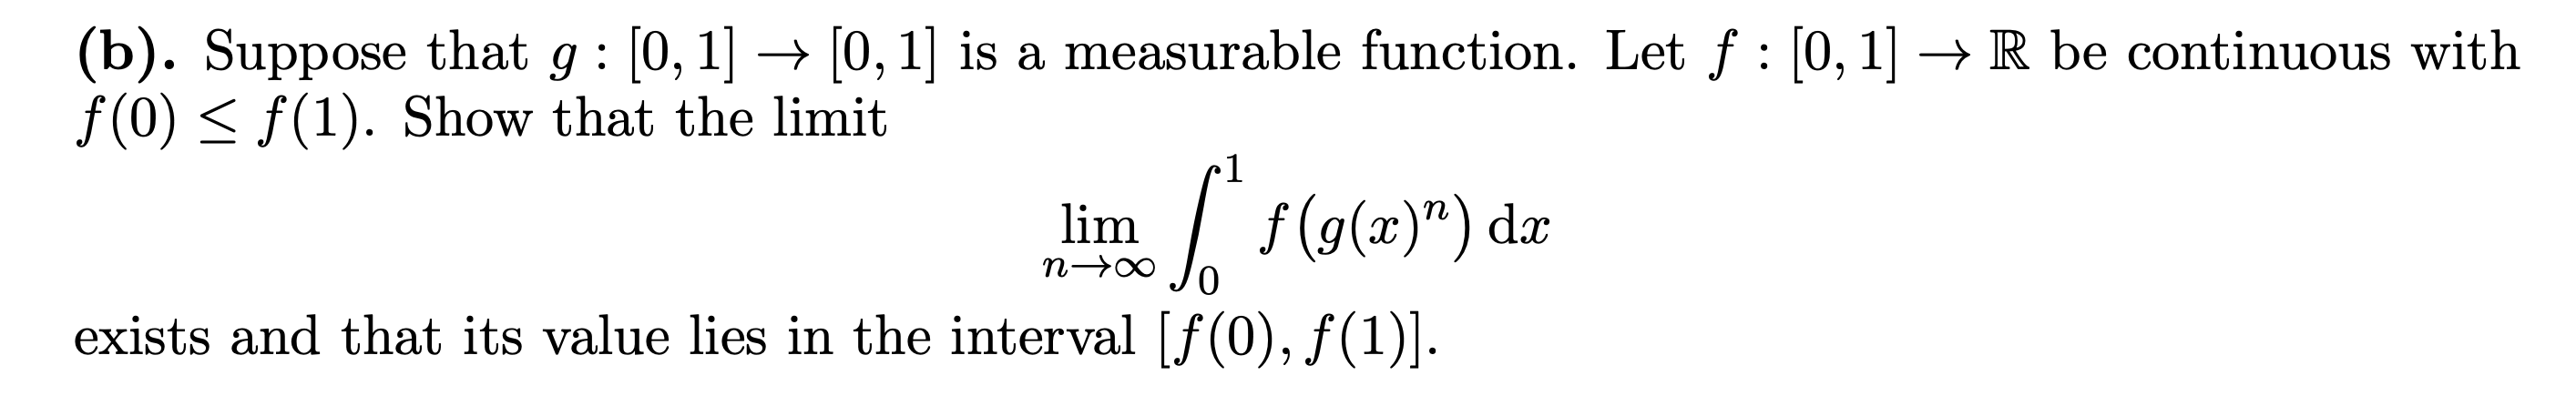
\includegraphics[width=400pt]{img/analysis--berkeley-202a-final-cd70.png}
\end{mdframed}
\green{COMPLETE}

\begin{proof}

  Note that $f$ is continuous with compact support and so $f$ attains its bounds. Let $A = \inf f$
  and $B = \sup f$.

  Note that the integrand is bounded above by the constant integrable function $h(x) = B$ defined on $[0, 1]$.
  Therefore we may apply the dominated convergence theorem, yielding
  \begin{align*}
    \limninf \int_{[0, 1]} f(g(x)^n) \dx = \int_{[0, 1]} \limninf  f(g(x)^n) \dx.
  \end{align*}
  Let $U = g^{-1}(\{1\})$. We have $0 \leq g(x) \leq 1$ and therefore
  \begin{align*}
    \limninf g(x)^n =
    \begin{cases}
      1 & x \in U \\
      0 & \text{otherwise}.
    \end{cases}
  \end{align*}
  Since $g$ is measurable, $U$ is measurable, since it is a preimage of a measurable set. Let $\alpha = m(U)$.
  I believe that ``measurable​'' in the question refers to Lebesgue measure, so we have that $m([0, 1]) = 1$
  and $0 \leq \alpha \leq 1$. Therefore
  \begin{align*}
    \int_{[0, 1]} \limninf  f(g(x)^n) \dx
    &= \int_U \limninf  f(g(x)^n) \dx + \int_{[0, 1] \setminus U} \limninf  f(g(x)^n) \dx \\
    &= \int_U f(1) + \int_{[0, 1] \setminus U} f(0) \\
    &= \alpha f(1) + (1 - \alpha) f(0) \\
    &\in [f(0), f(1)].
  \end{align*}
\end{proof}


\newpage
\begin{mdframed}
  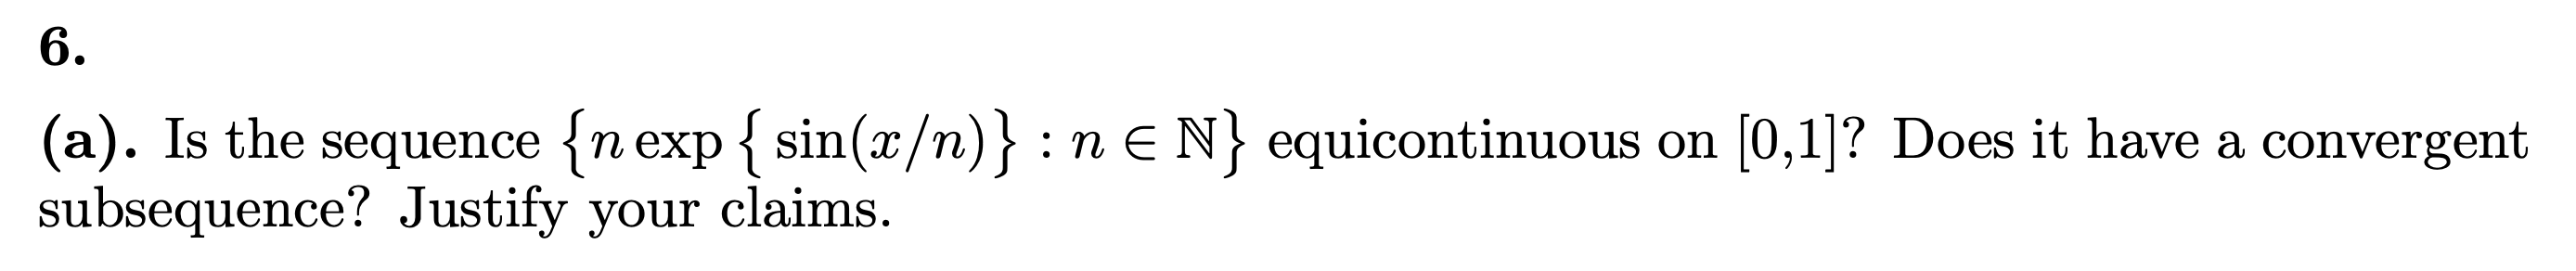
\includegraphics[width=400pt]{img/analysis--berkeley-202a-final-f5b6.png}
\end{mdframed}
\green{COMPLETE}

\begin{lemma}\label{bounded-derivative-implies-equicontinuous}
  Let $\mc F$ be a collection of functions, where $f: [0, 1] \to \R$ for every $f \in \mc F$. If
  the collection of derivatives $\{f' ~:~ f \in \mc F\}$ is uniformly bounded, then $\mc F$ is
  equicontinuous.
\end{lemma}

\begin{proof}
  Let $\eps > 0$ and suppose $|f'(x)| \leq M$ for all $x \in [0, 1]$ and all $f \in \mc F$.

  Let $x \in [0, 1]$ and let $G = (x - \frac{\eps}{2M} , x + \frac{\eps}{2M}) \isect [0, 1]$
  Then $G$ is open in $[0, 1]$ and we have $f(G) \subset (f(x) - \eps, f(x) + \eps)$ for
  all $f \in \mc F$. Therefore the family $\mc F$ is equicontinuous.
\end{proof}

\begin{claim*}
  The family $f_n$ is equicontinuous.
\end{claim*}

\begin{proof}
  Let $f_n = n \exp\{\sin(x/n)\}$ and let $\mc F = \{f_n ~:~ n \in \N\}$.

  Note that $f'_n(x) = \cos(x/n)\exp\{\sin(x/n)\}$, therefore $0 < f'_n(x) \leq 1$. I.e. $f'_n(x)$
  is uniformly bounded on $[0, 1]$. Therefore the family $f_n$ is equicontinuous by lemma
  \ref{bounded-derivative-implies-equicontinuous}.
\end{proof}

\begin{claim*}
  The family of functions $f_n$ does not have a convergent subsequence.
\end{claim*}

\begin{proof}
  For this question we consider the family of functions to be a metric space under the supremum
  norm. I.e. we define the distance between functions $f_n$ and $f_m$ to be
\begin{align*}
  d(f_n, f_m) = \origsup_{x \in [0, 1]} |f_n(x) - f_m(x)|.
\end{align*}
  Note that
  \begin{align*}
    f_{n+1}(x) - f_n(x) = (n + 1) \exp\{\sin(x/(n+1))\} - n \exp\{\sin(x/(n))\},
  \end{align*}
  therefore $\limninf \(f_{n+1}(x) - f_n(x)\) = 1$ for all $x \in [0, 1]$, and
  so $\limninf d(f_{n+1}, f_n) = 1$. Let $\eps_1 = 0.1$. Therefore there exists $N_1$ such
  that $d(f_{n + 1}, f_{n}) \in (1 - \eps_1, 1 + \eps_1) = (0.9, 1.1)$ for all $n \geq N_1$.

  Suppose for a contradiction that $f_{n_2}, f_{n_2}, \ldots$ converges to $g$,
  where $n_2 < n_2 < \cdots$. Therefore $f_{n_2}, f_{n_2}, \ldots$ is Cauchy. Let $N_2$ be such
  that $d(f_{n_i}, f_{n_j}) < \eps_2 = 0.5$ for all $i, j \geq N_2$ with $i \neq j$.

  But this is a contradiction since for $m = \max(N_1, N_2)$ we have both $d(f_{m}, f_{m+1}) < 0.5$
  and $d(f_{m}, f_{m+1}) \in (0.9, 1.1)$.

  Therefore $f_n$ does not have a convergent subsequence.
\end{proof}

\newpage
\begin{mdframed}
  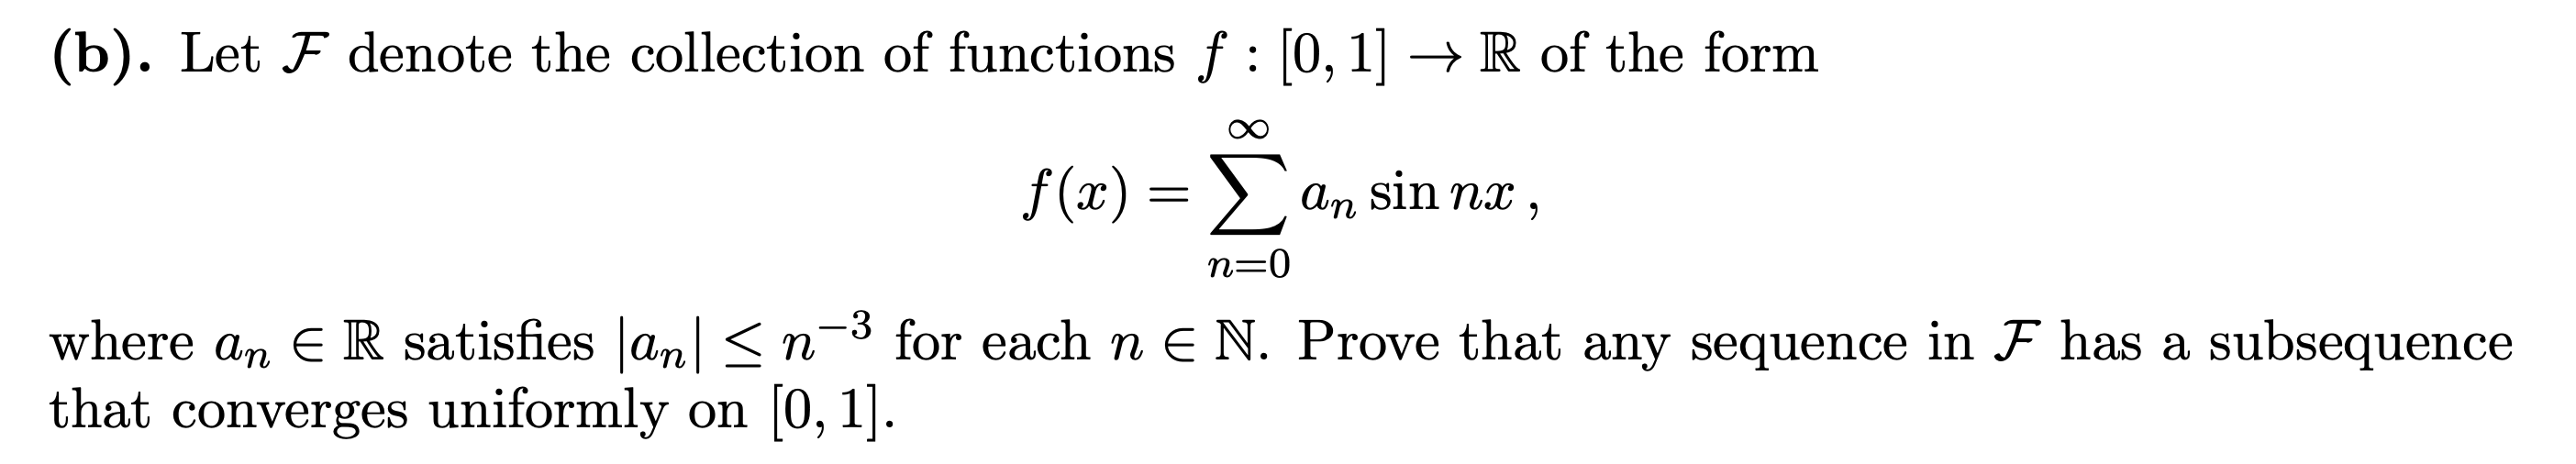
\includegraphics[width=400pt]{img/analysis--berkeley-202a-final-c7c7.png}
\end{mdframed}

% https://math.berkeley.edu/~vvdatar/m104su18/Assignments/Solutions_A7.pdf

\begin{remark*}
  In general, it is well-known from Fourier analysis that a discontinuous ``square wave​'' function
  can be written in the form $\sum_{n=0}^\infty a_n \sin nx$. Therefore it is not immediately
  obvious that every $f \in \mc F$ is continuous. On the other hand, here we are given a condition
  on the $a_n$ which might make every $f \in \mc F$ continuous. We will use this condition to prove
  that the conditions of the Ascoli - Arzelà theorem are indeed satisfied.
\end{remark*}

\begin{proof}
  Note that $[0, 1]$ with the topology induced by the standard Euclidean metric is compact and
  Hausdorff. Recall that (Bass p.249 remark after proof of Ascoli - Arzelà theorem) any sequence
  in $\mc F$ has a subsequence which converges uniformly on $[0, 1]$ if the following two
  conditions are met:
  \begin{enumerate}
  \item  $\origsup_{f \in \mc F} |f(x)| < \infty$ for all $x \in [0, 1]$
  \item $\mc F$ is equicontinuous (this implies that $\mc F \subseteq \mc C([0, 1])$).
  \end{enumerate}

  For the first condition, we have
  \begin{align*}
    |f(x)|
    =    \Big|\sum_{n=0}^\infty  a_n   \sin nx \Big|
    \leq      \sum_{n=0}^\infty |a_n| |\sin nx|
    \leq      \sum_{n=0}^\infty n^{-3}
    <         \infty
  \end{align*}
  for all $f \in \mc F$ and for all $x \in [0, 1]$.
  Therefore $\origsup_{f \in \mc F} |f(x)| < \infty$ for all $x \in [0, 1]$.

  For the second condition, note that $|a_n \sin nx| \leq n^{-3}$ for all $x \in [0, 1]$ and
  all $n \in \N$. Therefore, by the Weierstrass M-test, since $\sum_{n=0}^\infty n^{-3}$ is a
  convergent series, the series $\sum_{n=0}^\infty a_n \sin nx$ converges uniformly on $[0, 1]$,
  and it can be differentiated term by term. Thus we have
  \begin{align*}
    |f'(x)|
    =    \Big|\sum_{n=0}^\infty n a_n   \cos nx \Big|
    \leq      \sum_{n=0}^\infty n|a_n| |\cos nx|
    \leq      \sum_{n=0}^\infty n^{-2}
    <         \infty
  \end{align*}
  for all $f \in \mc F$. Therefore $\mc F$ is equicontinuous by lemma
  \ref{bounded-derivative-implies-equicontinuous}.

  Therefore any sequence in $\mc F$ has a subsequence which converges uniformly on $[0, 1]$.
\end{proof}


\newpage
\begin{mdframed}
  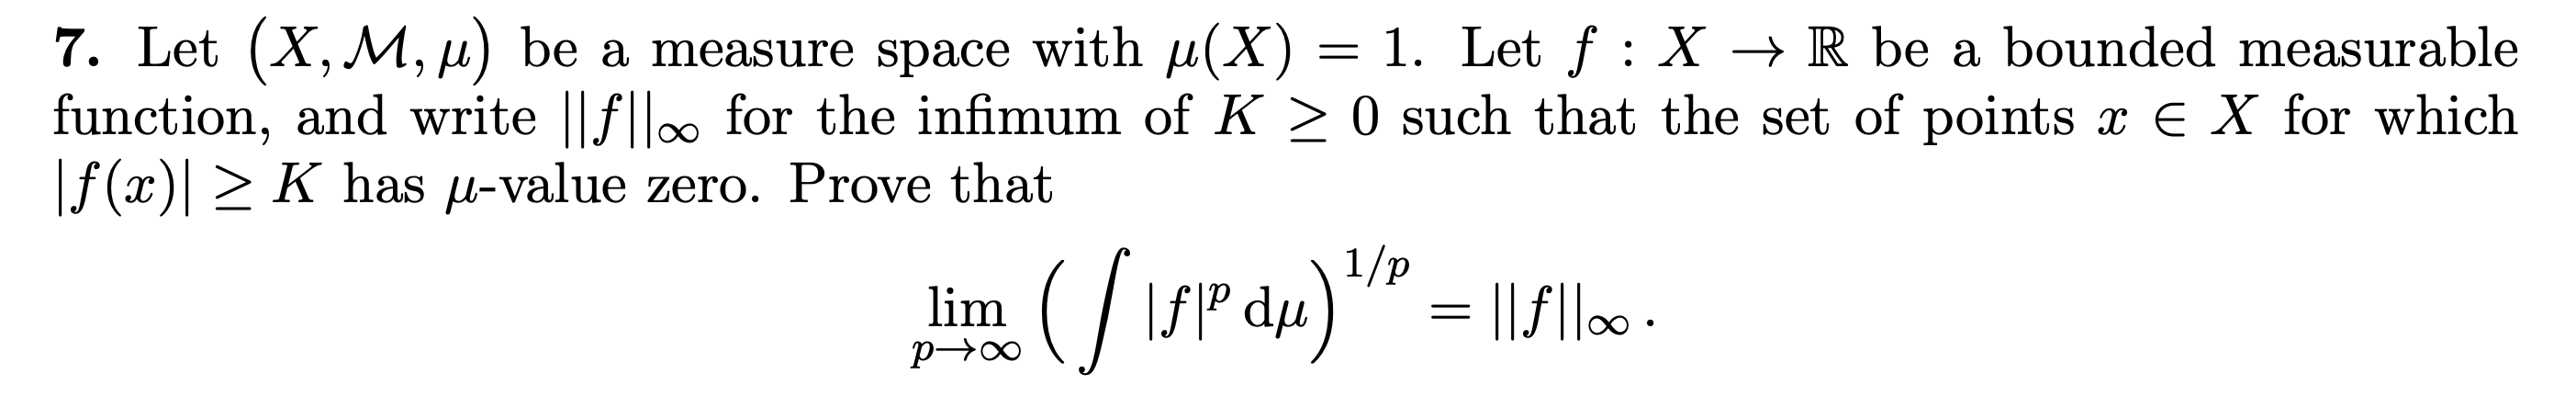
\includegraphics[width=400pt]{img/analysis--berkeley-202a-final-0000.png}
\end{mdframed}

% \begin{itemize}
% \item \url{https://www.wikiwand.com/en/Lp_space#/The_p-norm_in_infinite_dimensions_and_\%E2\%84\%93p_spaces}
% \item \url{https://www.wikiwand.com/en/Essential_supremum_and_essential_infimum}
% \item \url{https://math.stackexchange.com/questions/242779/limit-of-lp-norm}
% \item \url{https://math.stackexchange.com/questions/678884/if-f-in-l-infty-and-exists-r-infty-so-that-f-r-infty-show}
% \end{itemize}



% Let $A = \originf_{x \in X} f$ and let $B = \origsup_{x \in X} f$. Since $f$ is bounded these are both
% finite.

% Since $f$ is bounded, $|f|$ is bounded also. Let $B = \origsup_{x \in X} |f(x)|$. We
% have $\norm{f}_\infty \leq B$.

% As an example, let $f(x) = 0.9$ for all $x \in X$.
% Then $\(\int |f|^p \dmu\)^{1/p} = \(0.9^p\int 1 \dmu\)^{1/p} = 0.9$, so that is as expected.


\begin{proof}

  [incomplete]

  Let $L = \lim_{p \to \infty} \(\int |f|^p \dmu\)^{1/p}$.

  First consider $f$ simple, say $f = \sum_{j=1}^J a_j \ind_{E_j}$. Then
  \begin{align*}
    \int |f|^p \dmu = \sum_{j=1}^J |a_j|^p \mu(E_j)
  \end{align*}
  and (\red{TODO} proof)
  \begin{align*}
    \lim_{p \to \infty} \(\int |f|^p \dmu\)^{1/p}
    &= \max \Big\{|a_j| ~:~ \mu(E_j) > 0, j \in \{1, \ldots, J\}\Big\} \\
    &= \norm{f}_\infty.
  \end{align*}
  Next, consider $f$ measurable. Let $s_n$ be a sequence of simple functions increasing to $f$. Then
  \begin{align*}
    \int |f|^p \dmu = \lim_{n \to \infty}\sum_{j=1}^{J_n} |a_{nj}|^p \mu(E_{nj})
  \end{align*}

  First we will show that $L \geq \norm{f}_\infty$.

  Finally we show that $L \leq \norm{f}_\infty$.
  \red{TODO}
\end{proof}

I didn't get far with that. FWIW, here (\url{https://math.stackexchange.com/questions/242779/limit-of-lp-norm}) is a proof from
math.stackexchange. I obviously don't request any credit for this. I understand the $\geq$ part but
I would never have thought of that trick of creating a constant thing raised to the $p$-th power
inside the integral. The $\leq$ part uses Hölder's inequality I think, which I don't have any
intuition for.
\begin{mdframed}
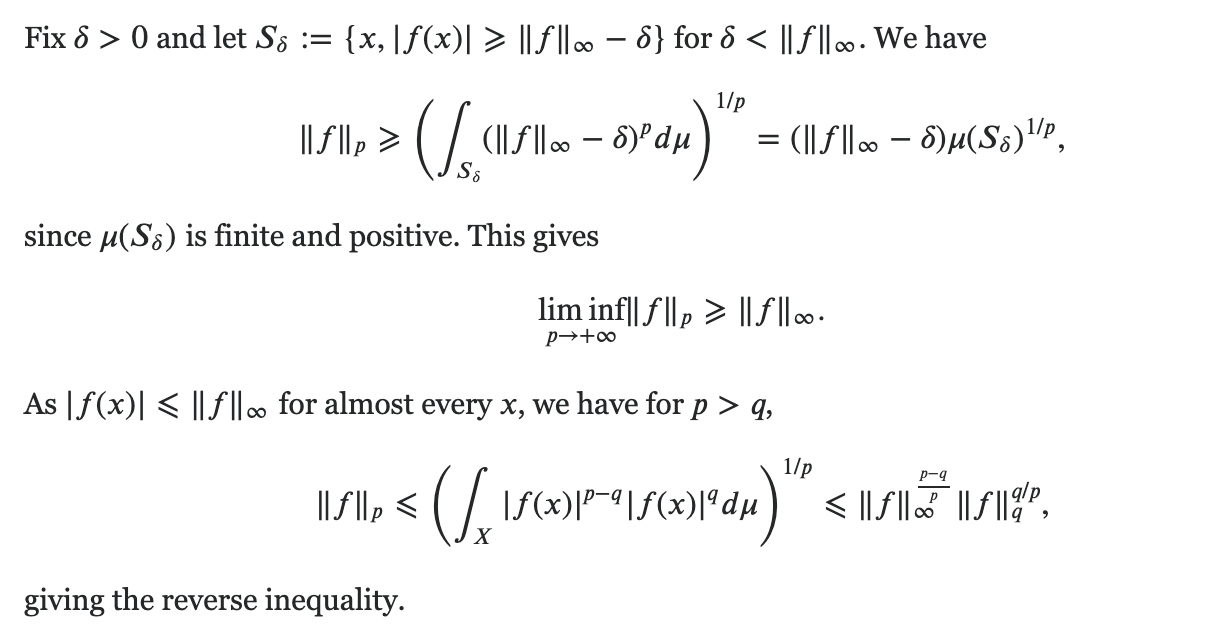
\includegraphics[width=300pt]{img/analysis--berkeley-202a-final-1b8f.png}
\end{mdframed}


\newpage
\begin{mdframed}
  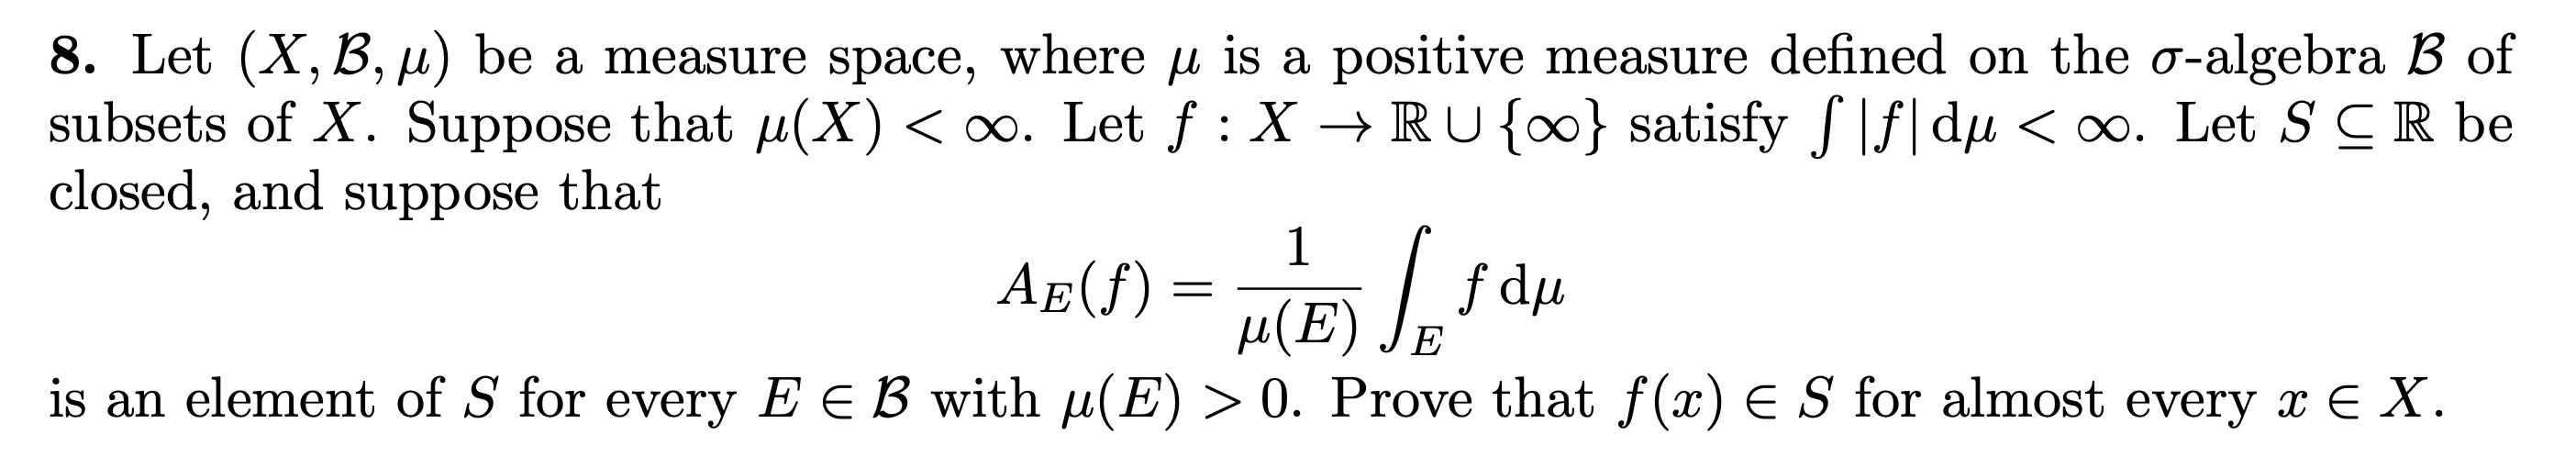
\includegraphics[width=400pt]{img/analysis--berkeley-202a-final-8aed.png}
\end{mdframed}

First, we prove this for $X = \R^n$.

\begin{proof}
  Since $f$ is integrable, it is locally integrable. So from Folland 3.18 we have
  that $\lim_{r \to 0} A_{B(x, r)}(f) = f(x)$ for a.e. $x$. Fix a real-valued sequence $r_n$ converging
  to $0$ from above. Then $A_{B(x, r_n)}(f)$ is a sequence in $S$ converging to $f(x)$. Since $S$
  is closed, it contains the limit of every convergent sequence in $S$, hence $f(x) \in S$ for
  almost every $x \in X$.
\end{proof}

\begin{remark*}
  This question involves an averaging construction similar to that associated with Hardy-Littlewood
  maximal function theory and the Lebesgue differentiation theorem (Folland section 3.4). However,
  the theory in Folland 3.4 concerns $\R^n$, whereas this question is about an abstract measure
  space. The theory in the Folland chapter requires the Vitali covering lemma, and so it seems to
  me that that is indeed completely tied to Euclidean space. Wikipedia
  (\url{https://en.wikipedia.org/wiki/Lebesgue_differentiation_theorem}) mentions that the Lebesgue differentiation theorem holds for
  a ``finite Borel measure on a separable metric space​'' obeying certain conditions, but we don't
  have a separable metric space.
\end{remark*}

Here's the beginnings of a proof for an abstract measure space, but I don't know how to complete
it.

\begin{proof}
  If $\mu(X) = 0$ then the result is trivially tru e so we assume $\mu(X) > 0$.

  We switch notation so that we now write $A_f(E)$ instead of $A_E(f)$, to emphasize that this is a
  set function, with the function $f$ a fixed parameter.

  We would like, for almost every $x$, to show that a sequence of sets $E_n$ exists such
  that $A_f(E_n) \to f(x)$ where $E_n \in \mc B$ and $\mu(E_n) > 0$ for all $n$. Then, since $S$ is
  closed, it contains the limit of every convergent sequence in $S$, and hence we will
  have $f(x) \in S$ for every $x \in X$.

  Let $E_n \downarrow \{x\}$. Then since $\mu(X) < \infty$ we have
  \begin{align*}
    \mu(\{x\}) = \limninf \mu(E_n)
  \end{align*}
  I don't know how to proceed.
\end{proof}

Some notes:
\begin{itemize}
\item We must use that $\mu(X) < \infty$.
\item We must use that $\int |f| \dmu < \infty$.
\item We are asked only for almost every $x \in X$
\item $\lambda(E) := \int_E f \dmu$ is a measure and $f$ is the Radon-Nikodym derivative of $\lambda$ with respect to $\mu$.
\item For a sequence of sets $E_n \downarrow \{x\}$ we have $\limninf \mu(E_n) = \mu(\{x\}) = 0$.
\item For a sequence of sets $E_n \downarrow \{x\}$ we have $\limninf \lambda(E_n) = \lambda(\{x\}) = 0$, since $\{x\}$ has measure zero.
\item We would like to show that $\mu(\{x ~:~ f(x) \text{~not the limit of the sequence of averages}\}) = 0$.
\end{itemize}


%%%%%%%%%%%%%%%%%%%%%%%%%%%%%%%%%%%%%%

% We have a finite measure space, and a single integrable function $f: X \to \R \union \{\infty\}$.

% Consider
% \begin{align*}
%   A_E(f) := \frac{1}{\mu(E)}\int_E f \dmu.
% \end{align*}
% We have that $\{A_E(f) ~:~ E \in \mc B\} \subseteq S$, where $S$ is a closed subset of $\R$.

% Note that $A_E(f) < \infty$.

% If we instead write $A_f(E)$, is this a measure?

% Let $E_1, \ldots$ partition $E$. Then
% \begin{align*}
%   A_f(E)
%   &= \frac{1}{\mu(E)}\int_E f \dmu \\
%   &= \frac{1}{\sumninf \mu(E_n)}\sumninf \int_{E_n} f \dmu.
% \end{align*}
% $A_f(E) = \sumninf \frac{\mu(E_i)}{\mu(E)} A_f(E_i)$.

% We have that for a sequence of decreasing sets $E_n \downarrow E$, if $\mu(E_1)$ is finite,
% then $\mu(E) = \limn \mu(E_n)$. So this may be why we are told that $\mu$ is finite.
